\section*{Union find%
\TAGS{union-find}}

We can answer the question of whether an edge creates a cycle by
tracking \emph{equivalence classes} of vertices. Two vertices are
equivalent if there's a path from one to the other using the spanning
tree edges we've already added during Kruskal's algorithm.

We use the \emph{union find} data structure to efficiently maintain
equivalence classes.  We think of union find as maintaining a
\emph{directed} graph called the \emph{equivalence graph}, where each
vertex has at most one outgoing edge, and where following a series of
directed edges eventually reaches the \emph{canonical representative}
of the equivalence class, which has no outgoing edge.

Two elements are equivalent if and only if they have the same
canonical representative. We can make two elements equivalent (when we
add an edge to the MST) by finding their canonical representatives and
connecting them with an edge.


\checkpoint*{\TAGS{spanning-tree, union-find}}

Run Kruskal's algorithm on the weighted graph to the left to form a
spanning tree. Track the structure of the equivalence graph to the
right. There's more than one answer.
\begin{center}
  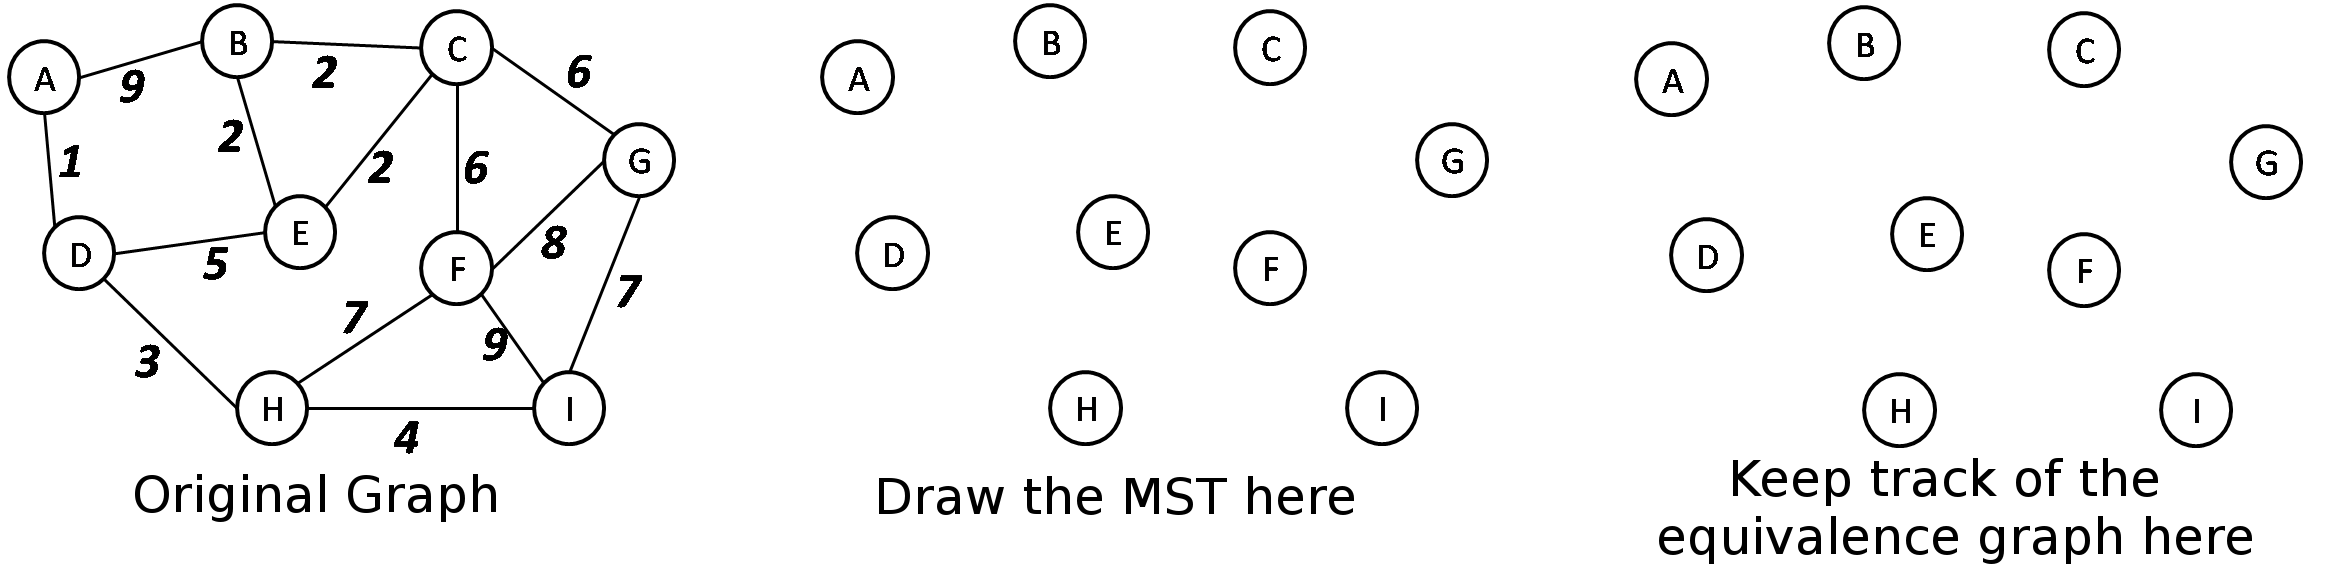
\includegraphics[width=0.91\textwidth]{\img/graph1_three_graphs.png}
\end{center}
Which edges that aren't even part of the original weighted graph end
up as directed edges in the equivalence graph?

\begin{solution}
There are only three total minimum spanning trees, depending
on which of BE, BC, and CE get excluded. There are a \emph{multitude}
of possible equivalence graphs, but if I did this right \emph{any}
equivalence graph must include one of the following directed edges:
AH, ID, HE, HB, or HC. None of these appear in the original
graph. Here are two examples:
\begin{center}
  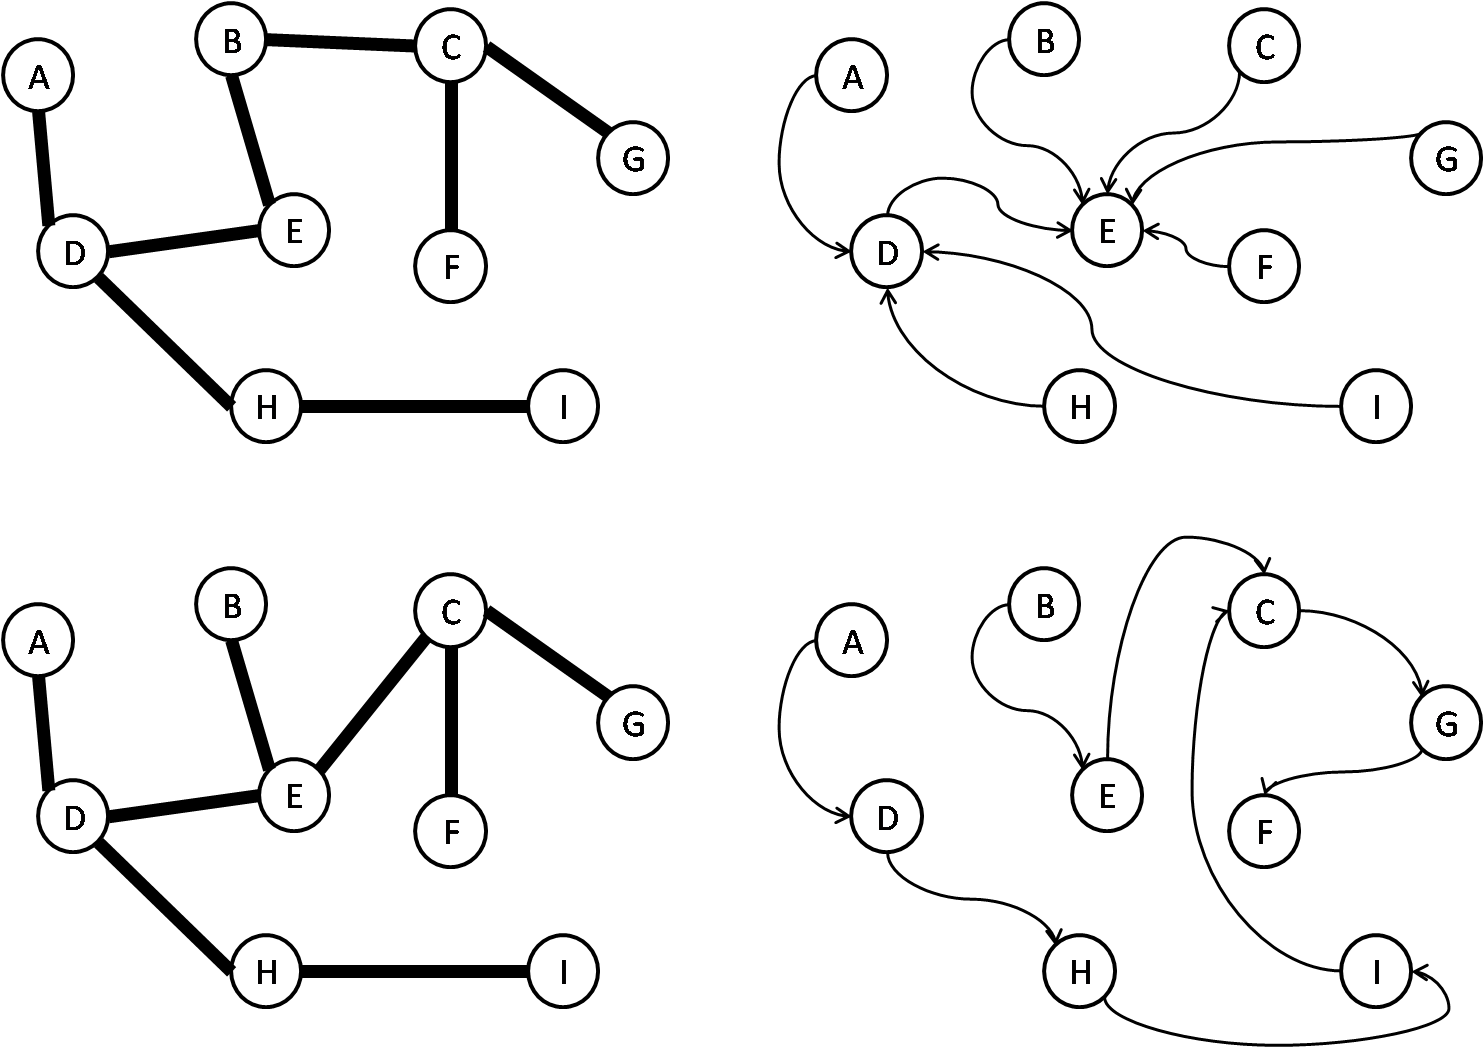
\includegraphics[width=.75\textwidth]{\img/graph1-sol.png}
\end{center}
\end{solution}
